\newpage
\section{Vorbereitungsfragen}
\subsection{Zeitlicher Verlauf der
drei Leistungsvariablen über den Zeitvektor t}
In \autoref{fig:plot3062023} ist der Leistungsverlauf der Last, des PV-Systems und die direkt verbrauchte PV-Systemleistung zu sehen.
\begin{figure}[H]
    \centering
    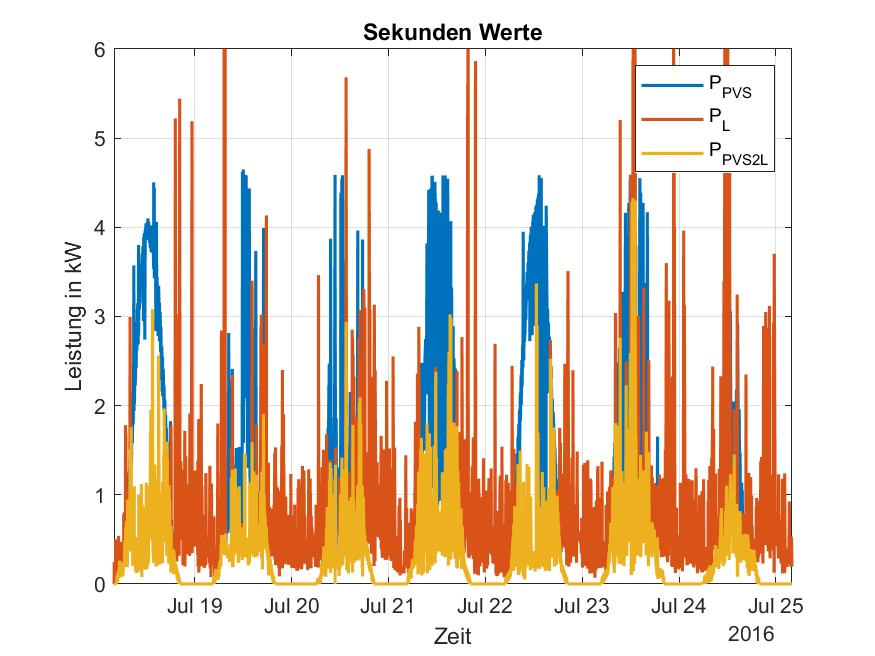
\includegraphics[width=\textwidth]{Abbildungen/plot.jpg}
    \caption{Zeitlicher Verlauf der drei Leistungsvariablen $P_{PVS}, P_{L}$ und $P_{PVS2L}$. Es handelt sich um Sekundenmittelwerte.}
    \label{fig:plot3062023}
\end{figure}
Es ist zu erkennen, dass es starke Tag und Nacht Fluktuationen gibt. 
Das bedeutet, dass die Höchstwerte immer zur Mittagszeit auftreten, die Leistung morgens ansteigt und abends wieder abfällt. Auch die elektrische Last weist übliche Muster auf, mit höheren Werten nachmittags bis abends. 
Wobei der direkte Verbrauch über den ganzen Tag verteilt ist mit einem Peak am mittag.

In \autoref{fig:plot1_2_3062023} sind die stündlichen Mittelwerte zu sehen.
\begin{figure}[H]
    \centering
    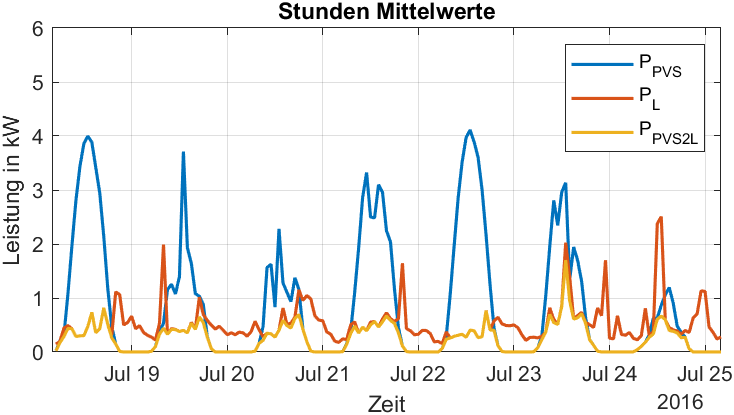
\includegraphics[width=\textwidth]{Abbildungen/aufgabe1_plot2.png}
    \caption{Zeitlicher Verlauf der drei Leistungsvariablen $P_{PVS}, P_{L}$ und $P_{PVS2L}$. Es handelt sich um Stundenmittelwerte.}
    \label{fig:plot1_2_3062023}
\end{figure}
Auch hier ist zu erkennen, dass das PV-System die Leistung, die am Tag benötigt wird, meistens sehr gut bereitstellen kann. Des Weiteren fällt auf, dass der Überschuss am Tag meistens sehr gro"s ausfällt und bis zu vier mal größer ist als der Leistungsbedraf der Last. Abends oder Nachts ist der Leistungsbedarf der Last nicht von der Leistung des Pv-Systems zu decken.
\subsection{Ermitteln Sie über den gesamten Messzeitraum die Energiesummen EPVS, EL und EPVS2L der
Leistungsvariablen PPVS, PL und PPVS2L (Angabe in kWh).}
Die zu ermittelnden Energiesummen lauten wie folgt:
\\
\textbf{Graph einfügen neu mit link vor der grafik!}

$E.E_pvs = sum(ts.Ppvs/1000)/3600=149,96kWh;\\
E.E_l = sum(ts.Pl/1000)/3600=89,08kWh;\\
E.E_pvs2l = sum(Ppvs2l/1000)/3600=41,52kWh;$\\

\subsection{Berechnung der Differenzleistung}
In \autoref{fig:plot3062023_2} ist die Differenz- sowie Batteriesystemleistung zu sehen.
\begin{figure}[H]
    \centering
    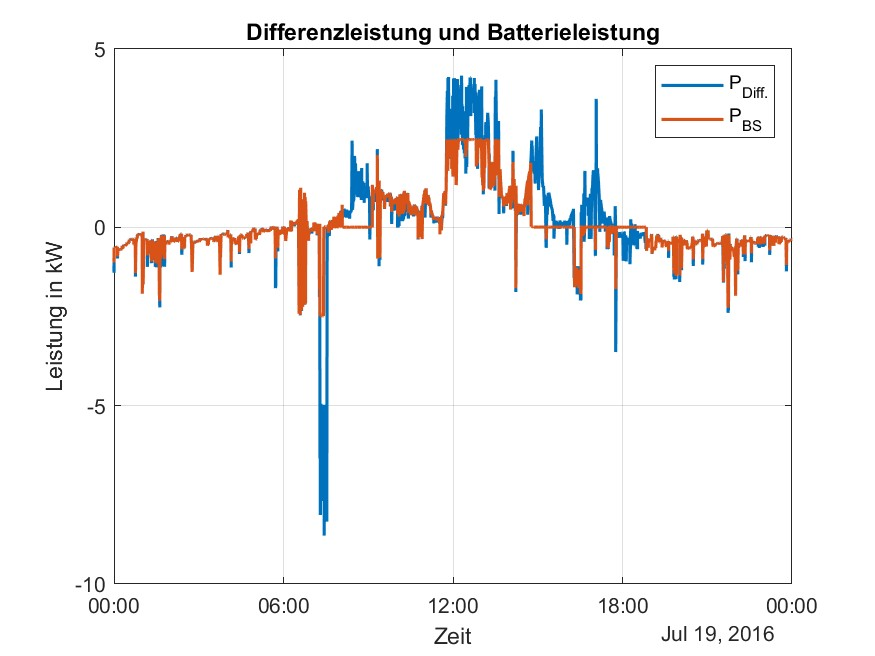
\includegraphics[width=\textwidth]{Abbildungen/plot_vorbereitungsfrage3.jpg}
    \caption{Differenzleistung und Batterieleistung im Vergleich}
    \label{fig:plot3062023_2}
\end{figure}
 
Die Batteriesystemleistung dient als Richtschnur, um festzustellen, ob es zu einem bestimmten Zeitpunkt geladen oder entladen wird. 
Eine positive Differenzleistung deutet auf einen Überschuss an Energie hin, wodurch das Batteriesystem aufgeladen werden kann, falls es nicht bereits vollständig geladen ist. Im Gegensatz dazu signalisiert eine negative Differenzleistung einen Energiemangel, der in erster Linie durch das Batteriesystem ausgeglichen werden sollte.
Dabei ist zu erkennen, dass die Differenzleistung größer ist als die Batterieleistung. 
Dies liegt daran, dass der Batteriespeicher nur eine endliche Menge an Leistung auf und abgeben kann.

\subsection{Funktionsweise des cumsum Befehls}

Der MATLAB-Befehl cumsum steht für cumulative sum und wird verwendet, um die kumulative Summe eines Vektors oder einer Matrix zu berechnen. 
Also statt die gesamte Summe zu berechnen, werden mit cumsum auch alle zwischen Summen gespeichert. In \autoref{fig:plot43062023} ist zu sehen, wie mithilfe des Befehls die Leistungen kumulierte werden und man eine Aussage über die kummulierte Einstrahlung erhält.
\begin{figure}[H]
    \centering
    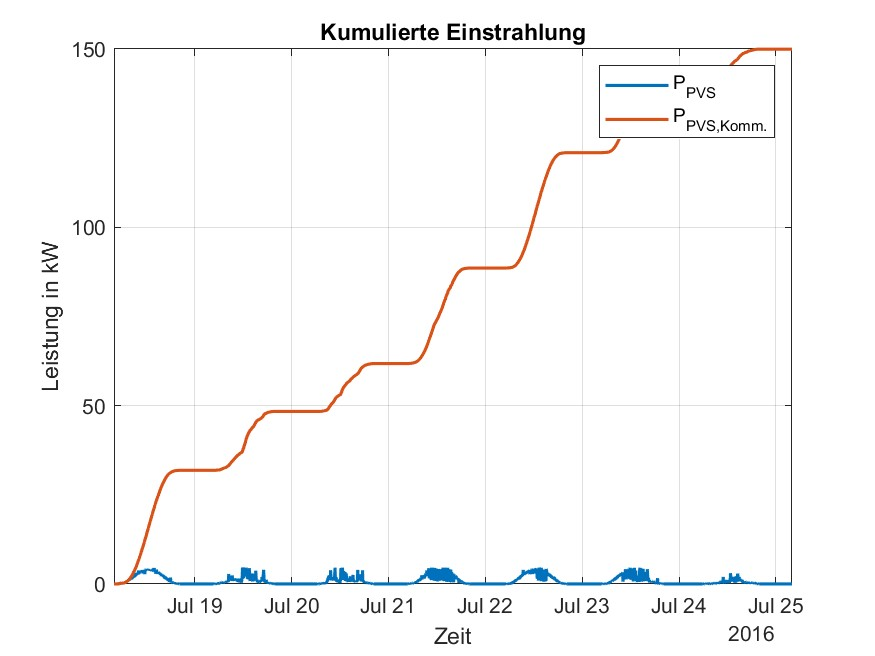
\includegraphics[width=\textwidth]{Abbildungen/plot_vorbereitungsfrage4.jpg}
    \caption{Anschauliche Darstellung des cumsum Befehls}
    \label{fig:plot43062023}
\end{figure}